\chapter{K\"ahler-Ricci solitons on Fano threefolds} \label{chap:sol}

\chaptermark{K\"ahler-Ricci solitons on Fano threefolds}


In this chapter we prove the following theorem:
\begin{theorem}[{\cite[Theorem 1.8]{cable2018classification}}] \label{thm:sol}
The Fano threefolds \(2.30, \ 2.31, \ 3.18, \ 3.22, \ 3.23, \ 3.24, \ 4.8\) from Mori and Mukai's classification \cite{mori1981classification} admit a non-trivial K\"ahler-Ricci soliton.
\end{theorem}
Together with \cite[Theorems. 6.1, 6.2]{ilten2015} it follows that all known smooth Fano threefolds with an effective complexity-one torus action admit a K\"ahler-Ricci soliton. We follow the joint work of \cite{cable2018classification}. We describe here the contribution of the author of this thesis to this article, namely to perform calculations to test the \(K\)-stability of threefolds and thus determine which admitted K\"ahler-Ricci solitons.

\section{The method of proof}
This proof of Theorem~\ref{thm:sol} is somewhat calculational in nature, and uses some computer assistance. We provide some context to our approach. At the end of this subsection we provide a more formal proof.

Let \(X\) be a smooth complexity one Fano \(T\)-variety. Recall the definition of a K\"ahler-Ricci soliton from definition \ref{def:tKRS}. We test for the existence of a K\"ahler-Ricci soliton on \(X\) using Theorem~\ref{thm:DS}. Recall from section~\ref{sec:toric} that the polarization \((X,-K_X)\) corresponds to a Fano divisorial polytope \(\Phi: \Box \to \Div \PP^1\), as defined in \ref{def:divpol}.

First we use Theorem \ref{thm:BWN} to find candidate vector fields \(\xi \in N_\RR\) for a soliton. By Theorem~\ref{thm:BWN}, any such \(\xi\) will satisfy the following equation: 
\begin{equation} \label{eq:producteq}
\DF_{\xi}(X \times \mathbb{A}^1, w) = 0.
\end{equation}
For all \(w \in N'_\RR\). By \ref{eq:futaki-character} this becomes:
\begin{equation} \label{eq:combproducteq}
\int_{\Box} \langle u, v \rangle \cdot \deg \bar \Phi(u) \cdot e^{\langle u, \xi \rangle}\, du = 0
\end{equation}
By the arguments in \cite[Section~3.1]{donaldson2008kahler} there always exist a unique choice $\xi \in N_\RR$ for which this holds. We refer to such a $\xi$ as a \textit{soliton canditate}.

The integral (\ref{eq:combproducteq}) may be solved symbolically, outputting an exponential polynomial \(g(\xi, e^{\xi})\) in \(\xi\). In practice however, the domain \(P\) can complicate the calculation for \(\dim X > 2\). To deal with this we developed a recursive algorithm, based on results of Barvinok \cite{Barvinok1992}, which reduces the integral to evaluations at the vertices of \(P\). We explain this algorithm at the end of this chapter.

For our examples the equation \(g(\xi,e^{\xi}) = 0\) is impossible to solve analytically. To get around this we use \textit{real interval arithmetic} (RIA) estimates to find some hypercube \(D\) in which the solution \(\xi\) lies. For each special test configuration \((\X,w)\) we then use further RIA to show that \(\DF_{\xi'}(\X,W)>0\) For \(\xi \in D\). In Table~\ref{table:solitontable} below we give estimates found for the vector field \(\xi\) for each threefold in the list of \cite{suss2013fano}. The threefolds 3.8*, 3.21, 4.5 were shown to admit a non-trivial K\"ahler-Ricci soliton in \cite{ilten2015}. We can show that our approximations are correct to the nearest \(10^{-5}\).

When \(\dim  X = 2\) the process of finding suitable \(D\) via RIA is a simple application of the intermediate value theorem. For \(\dim X >2 \) we cannot immediately use the intermediate value theorem to obtain \(D\). In all but one of our examples we make use of additional symmetries to reduce to a one-dimensional problem. Given an automorphism \(\sigma \in \GL(M)\) permuting the vertices of \(\Box\) such that \(\deg (\Phi \circ \sigma) = \deg \Phi\), by (\ref{eq:futaki-general-fibre}) we have:
\[
\DF_{X, \sigma^{\!*}\!(\xi)}  =  \DF_{X, \xi} \ \circ \ \sigma^*
\]

Since \(\xi \in N_\mathbb{R}\) is the unique solution to \(F_{X,\xi} = 0\), this gives \(\xi \in N_{\mathbb{R}}^{\sigma^*}\). For \(\dim X = 3\) we have \(\dim N_{\mathbb{R}}^{\sigma^*}  = 1\) and we are in a situation where intermediate value theorem may be used to find \(D\). Note that in threefold 3.23 there is no such involution, and we must take another approach, which we explain in the proof below and in Example~\ref{ex:assym}.
%
%
%
\begin{table}[H]  \centering
\captionsetup{width=.95\linewidth}
\caption{Fano threefolds and their soliton vector fields in the canonical coordinates coming with the representation of the combinatorial data in \cite{suss2013fano}.}  \label{table:solitontable}
\begin{tabular}{l l l}
\toprule
Threefold & $\xi$ & \\ \hline
Q & $(0,0)$ \\
2.24* & $(0,0)$ \\
2.29 & $(0,0)$ \\
2.30 & $(0,0.51489)$ \\
2.31 & $(0.28550,0.28550)$\\
2.32 & $(0,0)$ \\
3.8* & $(0,-0.76905)$ \\
3.10* & $(0,0)$ \\
3.18 & $(0,0.37970)$ \\
3.19 & $(0,0)$ \\
3.20 & $(0,0)$ \\
3.21 & $(-0.69622,-0.69622)$ \\
3.22 & $(0,0.91479)$ \\
3.23 & $(0.26618,  0.67164)$ \\
3.24 & $(0,0.43475)$ \\
4.4 &  $(0,0)$ \\
4.5* &  $(-0.31043,-0.31043)$ \\
4.7 &  $(0,0)$ \\
4.8 &  $(0,0.62431)$ \\
\bottomrule
\end{tabular}
\label{table:name}
\end{table}
We now give a more formal proof of Theorem~\ref{thm:sol}. The complete calculations for the proof are performed using SageMath, and can be found as an online worksheet\footnote{CoCalc:\url{https://cocalc.com/projects/ae8e1663-e2ad-40b8-aec2-30faf4e6a54f/files/threefolds.sagews}}.
\begin{proof}[Proof of Theorem~\ref{thm:sol}]
Note the data required for this proof is collated in Appendix~\ref{appendix1}. The divisorial polytopes were originally given in \cite{suss2013fano}, although the piecewise affine \(\Psi\) discussed there differs from our divisorial polytope \(\Phi\) by the divisor \(D = 2 \cdot \{ \infty \}\).

In threefolds 2.31, 3.18, 3.22, 3.24 and 4.8 there exists a non-trivial involution \(\sigma \in \GL(M)\) permuting the vertices of \(\Box\), such that \(\deg (\Phi \circ \sigma) = \deg \Phi\). Choose a basis $e_1, e_2$ of $N_\RR$ with $\sigma^*(e_1)=-e_1$ and $\sigma^*(e_2)=e_2$. The soliton candidate $\xi = (\xi_1,\xi_2)$ must be contained in the line $N_\RR^{\sigma^*} = \RR e_2$. For each of these example we obtain an interval \(D\) where the soliton candidate must lie, via the intermediate value theorem and RIA, see Appendix~\ref{appendix1}.

Recall the description of non-product special test configuration spaces from \ref{subsec:IS}. In Appendix~\ref{appendix1} we provide closed forms for \(h_y(\xi_2) := (\vol \Delta_y) \cdot \DF_{\xi_2 e_2}(\X,(0,1))\) for every admissible choice of $y \in \PP^1$. Recall by (ref) this is given by the integral
\begin{equation} \label{eq:specialDF}
\int
\end{equation}
using the algorithm described in \ref{sec:barvinok}. We also provide lower bounds on \(h_y(D)\) using further RIA, ensuring the positivity of $\DF_{\xi_2 e_2}(\X_{y,0,1})$. These threefolds then admit a K\"ahler-Ricci soliton by Theorem~\ref{thm:DS}. See Example~\ref{ex:sym} for details of the computation and Appendix~\ref{appendix2} for the implementation in SageMath.

For the case of threefold no. 3.23 there is no involution fixing $\deg \Phi$. In this case we take a more general approach to bound the value of the candidate \(\xi\). Here we make use of some elementary calculus. Note, that \(\xi\) is the unique solution to the equation \(\nabla_n G = 0 \), where 
\[
G(v) := \int_{\Box} \deg \bar \Phi(u) \cdot e^{\langle u, v \rangle}\, du = 
\int_{\Delta_0} e^{\langle u', (v,0) \rangle} \, du'.
\]
We identify a rectangular region \(D \subset \RR^2 \) such that \(\nabla_n G > 0 \) holds along \(\partial D\), where \(n\) is any unit outer normal of the rectangle \(D\). Since $D$ is compact it must contain a local minimum of $G$, which then cannot lie on \(\partial D\). We then have \(\xi\) in the interior of \(D\) such that \(\nabla_n G = 0\).

To show $\nabla_n G >0 $ along $\partial D$ we have to again use interval arithmetic. We determine a closed form which coincides with $\nabla_n G = \DF_\xi$ up to a positive constant. We subdivide the faces of the boundary into sufficiently small segments. Using RIA on the closed form for $\nabla_n G(\xi)$ we obtain the positivity result. See Example~\ref{ex:assym} for details of the computation and Appendix~\ref{appendix2} for the implementation in SageMath.
\end{proof}
\section{Two examples in detail}
Here we present threefolds 2.30 and 3.23 in detail:
\begin{example}[2.30 -- Blow up of quadric threefold in a point]
\label{exp:threefold}
Consider the threefold 2.30. The function \(\Phi\) is given in Figure~\ref{fig:data230}.
\begin{figure}[H]
\centering

\label{fig:data230b}
\resizebox{0.9\textwidth}{!}{
\begin{subfigure}[b]{0.25\linewidth}
\centering
  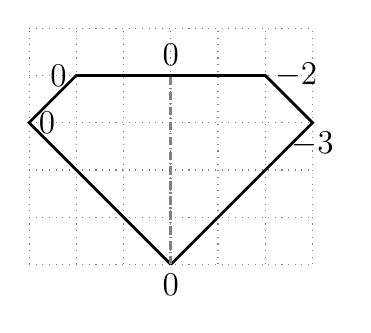
\begin{tikzpicture}[scale=0.6]
   	 \draw[dotted,step=1,gray,] (-3,-3) grid (3,2); \draw[line width = 1pt] (0,-3) --
     (-3,0) -- (-2,1)--(2,1)--
 	 (3,0)--(0,-3); \draw[densely dashdotted, gray, line width = 1.2pt] (0,-3) -- (0,1);
 	 \node at (0,-3) [below] {\large{$0$}};
 	 \node at (-3,0) [right] {\large{$0$}};
 	 \node at (-2,1) [left] {\large{$0$}};
 	 \node at (2,1) [right] {\large{$-2$}};
 	 \node at (3,0) [below] {\large{$-3$}};
 	 \node at (0,1) [above] {\large{$0$}};
	\end{tikzpicture}
	\caption*{$\Phi_0$}
\end{subfigure}
\begin{subfigure}[b]{0.25\linewidth}
	\centering
 	 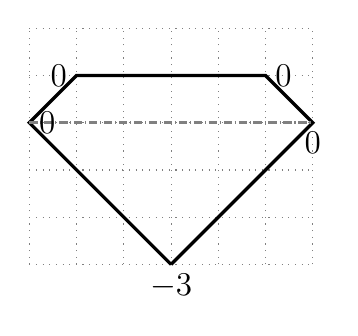
\begin{tikzpicture}[scale=0.6]
 	   \draw[dotted,step=1,gray] (-3,-3) grid (3,2); \draw[line width = 1.2pt] (0,-3) --
 	   (-3,0) -- (-2,1)--(2,1)--
 	   (3,0)--(0,-3); \draw[densely dashdotted, gray,line width = 1.2pt] (-3,0) -- (3,0);
 	 \node at (0,-3) [below] {\large{$-3$}};
 	 \node at (-3,0) [right] {\large{$0$}};
 	 \node at (-2,1) [left] {\large{$0$}};
 	 \node at (2,1) [right] {\large{$0$}};
 	 \node at (3,0) [below] {\large{$0$}};
	\end{tikzpicture}
	\caption*{$\Phi_1$}
\end{subfigure}
\begin{subfigure}[b]{0.25\linewidth}
	\centering
 	 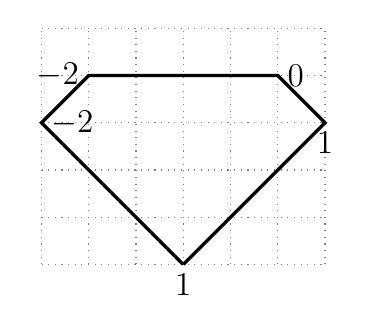
\begin{tikzpicture}[scale=0.6]
 	   \draw[dotted,step=1,gray] (-3,-3) grid (3,2); \draw[line width = 1.2pt] (0,-3) --
 	   (-3,0) -- (-2,1)--(2,1)--
 	   (3,0)--(0,-3);
 	 \node at (0,-3) [below] {\large{$1$}};
 	 \node at (-3,0) [right] {\large{$-2$}};
 	 \node at (-2,1) [left] {\large{$-2$}};
 	 \node at (2,1) [right] {\large{$0$}};
 	 \node at (3,0) [below] {\large{$1$}};
	\end{tikzpicture}
	\caption*{$\Phi_\infty$}
\end{subfigure}
\begin{subfigure}[b]{0.25\linewidth}
	\centering
 	 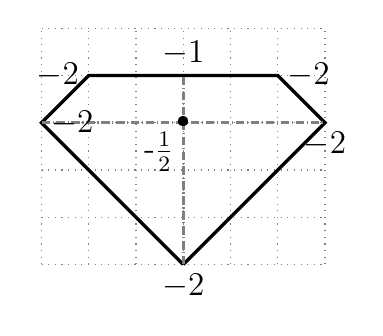
\begin{tikzpicture}[scale=0.6]
 	   \draw[dotted,step=1,gray] (-3,-3) grid (3,2); \draw[line width = 1.2pt] (0,-3) --
 	   (-3,0) -- (-2,1)--(2,1)--
 	   (3,0)--(0,-3); \draw[densely dashdotted, gray,line width = 1.2pt] (-3,0) -- (3,0); \draw[densely dashdotted, gray,line width = 1.2pt] (0,-3) -- (0,1) ;
 	 \node at (0,-3) [below] {\large{$-2$}};
 	 \node at (-3,0) [right] {\large{$-2$}};
 	 \node at (-2,1) [left] {\large{$-2$}};
 	 \node at (2,1) [right] {\large{$-2$}};
 	 \node at (3,0) [below] {\large{$-2$}};
 	 \node at (0,0) [below left] {\large{-$\frac{1}{2}$}};
 	 \node at (0,1) [above] {\large{$-1$}};
 	 \draw (0,0) node {\textbullet};
	\end{tikzpicture}
	\caption*{$\deg \Phi $}
\end{subfigure}
}
\end{figure}
We now find the unique candidate vector field \(\xi \in N_\mathbb{R}\) for a \(K\)-stable pair \((X,\xi)\). We see that $\deg \Phi$ is symmetric with respect to reflection $\sigma$ along the vertical axis. Hence, we have  \(\xi = \xi_2e_2\) for some \(\xi_2 \in \mathbb{R}\) and must find a solution $\xi_2$ to $F_{X,\xi_2e_2}=0$, which is equivalent to $F_{X,\xi_2e_2}(e_2)=0$. Indeed, we have 
\[F_{X,\xi_2e_2}(e_1) = F_{X,\sigma^*\xi_2e_2}(\sigma^*e_1)= F_{X,\xi_2e_2}(-e_1)= -F_{X,\xi_2e_2}(e_1).\]
Hence, $F_{X,\xi_2e_2}(e_1)=0$ and the claim follows by linearity.

By (\ref{eq:futaki-character}) the vanishing of $F_{X,\xi_2e_2}(e_2)$ is equivalent to that of
\[0=g(\xi_2) := \int_{\Box} u_2 \cdot \deg \bar \Phi(u) \cdot e^{u_2 \xi_2}\, du = \int_{\Delta_0} u_2 \cdot e^{u_2 \xi_2}\, du.\] Where the integral on the right hand side can be solved analytically. We obtain
\[
\frac{1}{\xi_{2}^{4}}\cdot\left({\left(2 \, \xi_{2}^{3} - 3 \, \xi_{2} - 3\right)} e^{\left(4 \, \xi_{2}\right)} + 12 \, \xi_{2} e^{\left(3 \, \xi_{2}\right)} + 3 \, \xi_{2} + 3\right) e^{\left(-3 \, \xi_{2}\right)}.
\]
Evaluating the exponential functions with a precision of 16 binary digits  and using elementary estimations it can be shown that \(g(0.514) <0\) and \(g(0.515)>0\). By the intermediate value theorem then \(0.514 < \xi_2 < 0.515\). It remains to check the positivity of the Donaldson-Futaki invariant for each degeneration. The degenerations of this threefold correspond to the polytopes:{
\begin{align*}
\Delta_0 &= \conv((-3,0,1),(-2,1,1),(2,1,-1),(3,0,-2),(0,-3,1),(0,1,1)); \\
\Delta_1 &= \conv((-3,0,1),(-2,1,1),(0,1,0),(2,1,1),(3,0,1),(0,-3,-2)); \\ 
\Delta_\infty &= \conv((-3,0,-1),(-2,1,-1),(2,1,1),(3,0,2),(0,-3,2),(0,0,-1),(0,1,-1)); \\
\Delta_y &= \conv((0, 0, -1/2), (3, 0, 1), (2, 1, 1), (0, 1, 0), (-2, 1, 1), (-3, 0, 1), (0, -3, 1)) \\ 
& \ \ \ ( \text{for } y 
\not \in \{0,1,\infty\} ).
\end{align*}}
In each case we have induced \(\CC^*\)-action given by \((0,0,1) \in N \times \ZZ \). Denote
\[
h_y(\xi_2) := (\vol \Delta_y) \cdot \DF_{(0,\xi_2)}(\X_{y,0,1}).
\]
Clearly positivity of \(h_y\) implies the positivity of \(\DF_\xi(\X_{y,0,1})\). 
Once more solving the integrals appearing in (\ref{eq:futaki-character}) analytically with $y \not \in \{0,1,\infty\}$  we obtain:
\begin{align*}
h_0(\xi_2) &= \frac{1}{3\xi_2^{4}}\cdot
{\left({\left(2   \xi_2^{3} - 3   \xi_2 - 3\right)} e^{4   \xi_2} + 3   {\left(3   \xi_2^{2} + 2\right)} e^{3   \xi_2} - 3   \xi_2 - 3\right)} e^{-3   \xi_2}
\\
h_1(\xi_2) &= \frac{1}{6   \xi_2^{4}}\cdot
{\left({\left(8   \xi_2^{3} + 6   \xi_2^{2} - 3\right)} e^{4   \xi_2} - 12   {\left(3   \xi_2^{2} - 3   \xi_2 + 1\right)} e^{3   \xi_2} + 12   \xi_2 + 15\right)} e^{-3   \xi_2} \\
h_\infty(\xi_2) &= -\frac{1}{6   \xi_2^{4}}\cdot
{\left(2   {\left(2   \xi_2^{3} - 3   \xi_2 - 3\right)} e^{4   \xi_2} - 3   {\left(3   \xi_2^{2} - 12   \xi_2 + 2\right)} e^{3   \xi_2} + 12   \xi_2 + 12\right)} e^{-3   \xi_2} \\
h_y(\xi_2) &= \frac{1}{6   \xi_2^{4}}\cdot{\left({\left(8   \xi_2^{3} + 6   \xi_2^{2} - 3\right)} e^{4   \xi_2 } - 3   {\left(3   \xi_2^{2} - 2\right)} e^{3   \xi_2} - 6   y - 3\right)} e^{-3   \xi_2} 
\end{align*}

Using the same precision as above for the  evaluations of the exponential functions at the lower and upper bounds for \(\xi_2\) gives estimates:
\begin{align*}
1.087 &< h_0(\xi_2) < 1.458 \\
2.178 &< h_1(\xi_2) < 2.470 \\
0.446 &< h_\infty(\xi_2) < 0.827 \\
4.151 &< h_y(\xi_2) < 4.309 \ \ \ \ \ \ \   \left( \text{for } y \not \in \{0,1,\infty\} \right)
\end{align*}
We can therefore conclude that the threefold 2.30 is \(K\)-stable, and must admit a non-trivial K\"ahler-Ricci soliton.
\end{example}

\begin{example}[3.23 -- Blowup of the quadric in a point and a line passing through]
\label{ex:assym}
We follow the calculations outlined in the above proof of Theorem~\ref{thm:sol}. As before we first have to find a closed form for $F_{X,\xi}(n)$ or $\nabla_n G(\xi)$, respectively. Then numerically we can find an approximation to \(\xi\) as the point:
\[
(x_0,x_1) = (0.26617786,  0.67164063).
\]
Setting \(\epsilon = 10^{-5}\), consider the square containing our approximation, given by:
\[
D = [x_0 - \epsilon,x_0+\epsilon] \times [x_1 - \epsilon, x_1 + \epsilon]
\]
Subdividing each edge of the boundary \(\partial D\) into line segments of length \(\epsilon/1500\), we use interval arithmetic to verify that the gradient of \(h\) is positive in the outer normal direction for each of these segments, in fact \(\nabla_n G > 5.536 \cdot 10^{-6}\) along \(\partial D\). Once again it remains to check the positivity of the Donaldson-Futaki invariant for each degeneration. The degenerations of this threefold correspond to the polytopes:
{
\
 \begin{align*}
\Delta_0 &= \conv((-3,0,1),(-2,1,1),(0,1,0),(0,1,1),(1,1,0),(2,0,-1),(2,-1,-1),\\
         &\qquad  (0,-3,1),(1,0,-1)); \\
\Delta_1 &= \conv((-3,0,1),(-2,1,1),(1,1,1),(2,0,1),(2,-1,0),(0,-3,-2),(0,1,0)); \\ 
\Delta_\infty &= \conv((-3,0,-1),(-2,1,-1),(0,1,0),(1,1,0),(2,0,1),(2,-1,2),(0,-3,2),\\
&\qquad (0,1,-1),(0,0,-1)) \\
\Delta_y &= \conv((0, 0, -1/2), (0, 1, 0), (1, 0, 0), (1, 1, 1), (2, 0, 1), (2, -1, 1), \\ & \qquad (-2, 1, 1), (-3, 0, 1), (0, -3, 1)) \ \ \  ( \text{for } y 
\not \in \{0,1,\infty\} ).
\end{align*}}
Interval arithmetic gives the following lower bounds on the Donaldson-Futaki invariants:
\begin{align*}
h_0(\xi_2) &> 1.2766 \\
h_1(\xi_2) &> 1.8401 \\
h_\infty(\xi_2) &> 0.1004 \\
h_y(\xi_2) &> 3.4443 \ \ \  ( \text{for } y 
\not \in \{0,1,\infty\} )
\end{align*}
We can therefore conclude that the threefold 3.23 is \(K\)-stable, and must admit a non-trivial K\"ahler-Ricci soliton. See also Appendix~\ref{App:code} for the SageMath code of the calculations.
\end{example}

\section{Barvinok Integration} \label{sec:barvinok}
The integrals \ref{eq:combproducteq}, \ref{eq:specialDF} may be solved symbolically, outputting exponential polynomials in the variable \(\xi\). In practice, the domain \(\Box\) can complicate these calculations for \(\dim X > 2\). To deal with this we developed a recursive algorithm, using results of Barvinok \cite{Barvinok1992}, which reduces the integral to evaluations at the vertices of \(\Box\).

We are interested in integrals of the following form:
\begin{equation} \label{eq:barintegral1}
\int_{P} l_1(x) e^{l_2(x)}
\end{equation}
for some linear functions \(l_1,l_2\) and some polytope \(P\). If we were working with surfaces, as is done earlier in \cite{cable2018classification}, then \(P\) is just an interval and the integral can be computed easily by hand. In theory, one could subdivide and parameterize the domain for higher dimensions, but this quickly makes the process of integration a very time-consuming and computation-heavy task, for even mildly complicated \(P\).

In \cite{barvinok}, Stoke's theorem is applied to a polytope domain to obtain formulae for integrals of a similar form. In particular we make use of the following:
\begin{lemma}[\cite{Barvinok1992}] \label{lem:bar}
Let \(\{\Gamma_i\}_i\) be the set of all facets of a polytope \(P\) and \(\mu_i\) be the Lebesgue measure on the affine hull of \(\Gamma_i\) induced from \(dx\) on \(\RR^n\). Denote by \(n_i\) the outer unit normal to \(\Gamma_i\). Let \(c \in \CC^n\) and \(\Lambda \in \RR^n\) such that \(\langle \lambda, c \rangle \neq 0\). Then
\begin{equation} \label{eq:barv}
\int_P e^{\langle c, x \rangle} dx = \frac{1}{\langle c , \lambda \rangle} \sum_i   \langle n_i, \lambda \rangle \int_{\Gamma_i} e^{\langle c, x \rangle} d \mu_i.
\end{equation}
\end{lemma}
We now outline how we implement this in the form of a recursive algorithm. Care must be taken to ensure the correct scaling is used when applying Lemma~\ref{} with induced Duistermaat Heckmann measures \(\nu_i\) instead of induced Lebesgue measures \(\mu_i\), but this amounts to using lattice-primitive normals rather than Lebesgue unit normals. We will only describe how our algorithm works for \(l_1 = 1\), as the general case may be obtained through integration by parts.

First we describe certain constructions needed in the recursion process. Any facet \(F\) of a polytope \(P\) is given by some equation \(\langle a, x \rangle = \langle a, u_0 \rangle \) for some primitive element \(a \in N\) and a choice of vertex \(u_0 \in \Vert(F)\). Consider the sublattice \(M_F := \ker a\). Denote the inclusion \(\iota:M_F \to M\), and pick a section \(s: M \to M_F\) of \(\iota\), given by a matrix with rows forming a basis of primitive lattice elements of \(M_F\). We may identify \(F \cong P_F := F - u_0\). Set \(c_F = \iota^*(c)\), and \(\lambda_F = s(\lambda)\).

We can now use the formula \ref{eq:barv} to define a recursive function \(\text{Barv}\) to compute the integral \(\int_P e^{ \langle c , \rangle x} dx\). It takes input \((N,F,c,\lambda)\). We have the following relation:
\[
\text{Barv}(M,F,c,\lambda) = \sum_F \frac{e^{\langle c, u_0 \rangle} }{\langle c, \lambda \rangle} \cdot \langle \lambda, n_F \rangle \text{Barv}(M_F, P_F,c_F,\lambda_F)
\]
We give our algorithm in pseudocode below.
\IncMargin{1em}
\begin{algorithm}[h] \label{alg1}
\SetKwInOut{Input}{input}\SetKwInOut{Output}{output}
\Input{A tuple \((N,P,c,\lambda)\) as described above, with \(\lambda\) sufficiently general.}
\Output{The integral \(\int_P e^{\langle c, x \rangle} dx\)}
\BlankLine
\(I \leftarrow 0\)\;
\eIf{\(c = 0\)}{
   \eIf{\(\dim P = 0\)}{
   \Return \(1\)\;
   }{
   \Return \(\vol_{\nu_P}(P)\)\;
   }
   }{
\For{\(F\) a facet of \(P\)}{
\(u_0 \leftarrow\) a vertex of \(F\)\;
\(M_F \leftarrow\) the ambient lattice of \(F\)\;
\(n_F \leftarrow\) the primitive outer normal to \(M_F\)\;
\(s \leftarrow\) an appropriate section of \(M_F \subset M\)\;
\(P_F \leftarrow F - u_0\)\;
\(c_F \leftarrow \iota^*(c)\)\;
\(\lambda_F \leftarrow s(\lambda)\)\;
\(\text{coeff}_F \leftarrow \frac{e^{\langle c, u_0 \rangle} }{\langle c, \lambda \rangle} \cdot \langle \lambda, n_F \rangle\)\;
\(I \leftarrow I + \text{coeff} \cdot \text{Barvinok}(N_F,P_F,c_F,\lambda_F)\)\;
}
}
\Return I
\caption{\(\text{Barv}(M,P,c,\lambda)\)}\label{algo_disjdecomp}
\end{algorithm}
Caching was later added, by S\"u\ss, to reduce computation time. The full SageMath code is included in \ref{appendix2}.
\newpage
We now describe one branch of the recursion for a simple 2-dimensional example. 
\begin{example}
Suppose \(P = \conv( \{ (\pm 1, \pm 1)\}), c = (0,1)\). We have facets \(F_1,\dots,F_4\) as labelled in \ref{}. In this case \(\lambda = (1,1)\) is clearly sufficiently general.

\begin{figure}[H]
\centering
\begin{subfigure}[b]{0.5\linewidth}
	\centering
 	 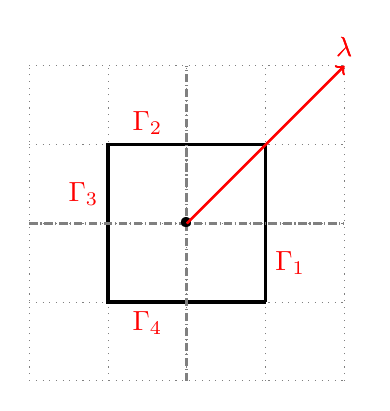
\begin{tikzpicture}[scale=1]
 	   \draw[dotted,step=1,gray] (-2,-2) grid (2,2); \draw[line width = 1.2pt] (1,-1) --
 	   (1,1) -- (-1,1)--(-1,-1)--
 	   (1,-1);
 	   \draw[densely dashdotted, gray,line width = 1.2pt] (-2,0) -- (2,0); \draw[densely dashdotted, gray,line width = 1.2pt] (0,-2) -- (0,2) ;
 	 \draw (0,0) node {\textbullet};
 	 \draw[red,->,thick] (0,0) -- (2,2);
 	 \node at (2,2) [above,red] {{$\lambda$}};
 	 \node at (1,-1/2) [right,red] {{$\Gamma_1$}};
 	 \node at (-1/2,1) [above,red] {{$\Gamma_2$}};
 	 \node at (-1,3/8) [left,red] {{$\Gamma_3$}};
 	 \node at (-1/2,-1) [below,red] {{$\Gamma_4$}};
 	 \draw[red,->,thick] (0,0) -- (2,2);
 	 \node at (2,2) [above,red] {{$\lambda$}};
	\end{tikzpicture}
	\end{subfigure}
\begin{subfigure}[b]{0.25\linewidth}
	\centering
 	 \begin{tikzpicture}[scale=1]
 	 \draw[dotted,step=1,gray] (-2,-2) grid (2,2);
 	 \draw (0,0) node {\textbullet};
 	 \draw[red,->,thick] (0,0) -- (0,1);
 	 \node at (0,1) [above,red] {\large{$c$}};
	\end{tikzpicture}
\end{subfigure}
\end{figure}
The first face we consider is \(F_1\). We pick \(u_0 = (1,-1)\), and we have \(M_F = \ZZ, \ n_F = (1,0)\). Pick \(s = (0,1)\). Now \(P_{F_1} = [0,2] \subset M_F \otimes \RR\), \(c_F = 1\), \(\lambda_F = 1\). We calculate \(\text{coeff}_F = e^{-1}\).
\begin{figure}[H]
\centering
\begin{subfigure}[b]{0.25\linewidth}
	\centering
 	 \begin{tikzpicture}[scale=1]
 	 \draw[dotted,step=1,gray] (0,-1) -- (0,3);
 	 \draw[line width = 1.2pt] (0,0) -- (0,2);
 	 \draw (0,0) node {\textbullet};
 	 \draw (0,2) node {\tiny{\textbullet}};
 	 \node at (0,1) [right,red] {{$P_{F_1}$}};
 	 \draw[->] (0,0) -- (0,1);
 	 \node at (0,1) [left] {{$\lambda_{F_1}$}};
	\end{tikzpicture}
\end{subfigure}
\begin{subfigure}[b]{0.25\linewidth}
	\centering
 	 \begin{tikzpicture}[scale=1]
 	 \draw[dotted,step=1,gray] (0,-1) -- (0,3);
 	 \draw[->] (0,0) -- (0,1);
 	 \node at (0,1) [above] {{$c_{F_1}$}};
 	 \draw (0,0) node {\textbullet};
	\end{tikzpicture}
\end{subfigure}
\end{figure}
On this branch it remains to calculate \(\text{Barv}(M_F,P_F,c_F,\lambda_F) = \int_0^2 e^x dx\). Applying the algorithm again We obtain \(e^2 - e\). In sum then \(F_1\) contributes \(e^{-1}*(e^2-e) = e-1\) to the overall integral \(\int_P e^y dx\).
\end{example}